% Copyright (C) 2005-2015 Airbus - EDF - IMACS - Phimeca
% Permission is granted to copy, distribute and/or modify this document
% under the terms of the GNU Free Documentation License, Version 1.2
% or any later version published by the Free Software Foundation;
% with no Invariant Sections, no Front-Cover Texts, and no Back-Cover
% Texts.  A copy of the license is included in the section entitled "GNU
% Free Documentation License".

This section provides informations on how to develop within the perimeter of the library and it's documentation.

\newcounter{oldenumi}

\subsection{Install a development version of OpenTURNS}

\subsubsection{Install the required dependencies}

See \ref{tools}, for the system requirements.

\subsubsection{Download openturns}

You can retrieve the development master branch through the scm repository by issuing the following command:
\begin{lstlisting}
svn co https://svn.openturns.org/openturns/trunk
cd trunk
\end{lstlisting}

Or, you can pick up a stable version tarball:
\begin{lstlisting}
wget http://downloads.sourceforge.net/openturns/openturns/openturns-1.1.tar.bz2
tar xjf openturns-1.1.tar.bz2
cd openturns-1.1
\end{lstlisting}

You may want to install the provided R package enabling additional statistical capabilities:
\begin{lstlisting}
R CMD INSTALL utils/rot_1.4.5.tar.gz
\end{lstlisting}

You can verify it's correct installation by typing:
\begin{lstlisting}
R --vanilla <<< 'library(rot)'
\end{lstlisting}

\subsubsection{Build openturns}

\begin{lstlisting}
mkdir build
cd build
cmake -DCMAKE_INSTALL_PREFIX=$PWD/install ..
make install -j4
\end{lstlisting}

\subsubsection{Run tests}
\begin{lstlisting}
make tests
ctest -j4
\end{lstlisting}
and all the tests should be successful else check the log file Testing/Temporary/LastTest.log.

\subsection{Adding a class to an existing directory \label{SingleClass}}

This how-to explains the process that must be followed to fully integrate a new class that provides an end-user facility (e.g. a new distribution). We suppose that this class will take place in an existing directory of the sources directories.

\subsubsection{First, add the class to the \OT\ C++ library}


\begin{enumerate}
\item Create \verb!MyClass.hxx! and \verb!MyClass.cxx! in the same directory. The files must have the standard header comment, with a brief description of the class in Doxygen form and the standard reference to the LGPL license.

For the header file \verb!MyClass.hxx!, the interface must be embraced between the preprocessing clauses:

\begin{lstlisting}
#ifndef OPENTURNS_MYCLASS_HXX
#define OPENTURNS_MYCLASS_HXX

BEGIN_NAMESPACE_OPENTURNS

class OT_API MyClass
{
CLASSNAME;

public:
  // default constructor
  MyClass();
...
};

END_NAMESPACE_OPENTURNS

#endif // OPENTURNS_MYCLASS_HXX
\end{lstlisting}

to prevent from multiple inclusions.

See any pair of .hxx/.cxx files in the current directory and the PGQL document for the \OT\ coding rules: case convention for the static methods, the methods and the attributes, trailing underscore for the attribute names for naming a few.

\item Modify the \verb!CMakeLists.txt! file in the directory containing \verb!MyClass.hxx! and \verb!MyClass.cxx!:
\begin{itemize}
\item add \verb!MyClass.hxx! to the headers using \verb!ot_install_header_file ( MyClass.hxx )!.
\item add \verb!MyClass.cxx! to the sources using \verb!ot_add_source_file ( MyClass.cxx )!.
\end{itemize}

\item Add \verb!MyClass.hxx! to the file \verb!OTXXXXXX.hxx!, where \verb!XXXXXX! is the name of the current directory.

\item Create a test file \verb!t_MyClass_std.cxx! in the directory lib/test. This test file must use the standard functionalities of the class MyClass.

\item Create an expected output file \verb!t_MyClass_std.expout! that contains a verbatim copy of the expected output (copy-paste the \emph{validated} output of the test in this file).

\item Modify the \verb!CMakeLists.txt! file in lib/test: add \verb!ot_check_test ( MyClass_std )! in this file.

\item If the validation of your class involved advanced mathematics, or was a significant work using other tools, you can add this validation in the validation/src directory.
\begin{itemize}
\item copy all of your files in the validation/src directory.
\item modify the validation/src/CMakeLists.txt file by appending the list of your files to the list of files to install.
\end{itemize}
\setcounter{oldenumi}{\value{enumi}}
\end{enumerate}

That's it! Your class is integrated to the library and will be checked for non-regression in all the subsequent versions of OpenTURNS, assuming that your contribution has been incorporated in the "official" \OT\ release. But nobody can use it!

\subsubsection{Second, add your class to the Python interface}

\begin{enumerate}
\setcounter{enumi}{\value{oldenumi}}
\item Create MyClass.i in the python/src directory. In most situations, it should be:
\begin{lstlisting}
// SWIG file MyClass.i
// Author: $LastChangedBy: schueller $
// Date: $LastChangedDate: 2012-02-27 14:48:06 +0100 (Mon 27 Feb 2012) $
// Id: $Id: MyClass.i 1539 2012-02-27 13:48:06Z schueller $

%{
#include "MyClass.hxx"
%}

%include MyClass_doc.i

%include MyClass.hxx
namespace OT {
%extend MyClass {

MyClass(const MyClass & other)
{
return new OT::MyClass(other);
}

} // MyClass
} // OT
\end{lstlisting}

\item Create MyClass\_doc.i.in docstring documentation in the python/src directory. This will be part of the HTML documentation generated by sphinx.
Document every method of your class that's not inherited. In most situations, it should look like this:

\begin{lstlisting}
%feature("docstring") OT::MyClass
"MyClass class.

Available constructors:
    MyClass()

    MyClass(*designPoint, limitStateVariable, isInFailureSpace*)

Notes
-----
Structure created by the method run() of a :class:`~openturns.Analytical`
and obtained thanks to the method *getAnalyticalResult*.

Parameters
----------
designPoint : float sequence
    Design point in the standard space resulting from the optimization
    algorithm.
limitStateVariable : :class:`~openturns.Event`
    Event of which the probability is calculated.
isInFailureSpace : bool
    Indicates whether the origin of the standard space is in the failure space.

Examples
--------
>>> import openturns as ot
>>> dp = ot.Normal().getRealization()
>>> inst = ot.MyClass(dp, 4.8)
>>> print(inst)"

// ---------------------------------------------------------------------

%feature("docstring") OT::MyClass::foo_method
"...
"

// ---------------------------------------------------------------------

...
\end{lstlisting}

\item Modify the CMakeLists.txt file in python/src: add MyClass.i, MyClass\_doc.i.in to the relevant \verb!ot_add_python_module! clause.

\item Locate and modify the file yyyy.i, where yyyy is the name of the python module related to MyClass, to include MyClass.i in the correct set of .i files (see the comments in yyyy.i file). In order to identify the correct python module, remember that the modules map quite closely the source tree organization.

\item Create a test file \verb!t_MyClass_std.py! in the directory python/test. This test implements the same tests than \verb!t_MyClass_std.cxx!, but using python.

\item Modify the CMakeLists.txt file in python/test:
\begin{itemize}
\item add \verb!t_MyClass_std.py! to the tests using \verb!ot_pyinstallcheck_test ( MyClass_std )!.
\end{itemize}
\setcounter{oldenumi}{\value{enumi}}
\end{enumerate}

\subsubsection{Document your contribution more thoroughly}

If your class introduces important mathematical concepts or impacts the library architecture it may be useful to add some more details in the latex documentation.

\begin{enumerate}
\setcounter{enumi}{\value{oldenumi}}

\item Build and download the documentation:
\begin{lstlisting}
svn co https://svn.openturns.org/openturns-doc/trunk
cd trunk
mkdir build
cd build
cmake -DCMAKE_INSTALL_PREFIX=$PWD/install \
-DOpenTURNS_DIR=OT_PREFIX/lib/cmake/openturns ..
make
make install
make check
\end{lstlisting}

\item Add an entry in the document src/DevelopersGuide/OpenTURNS\_DevelopersGuide.tex if your class has a significant impact on the library architecture or if your class has a significant impact on the way \OT\ interfaces external codes.

\item Add an entry in the document src/ReferenceGuide/OpenTURNS\_ReferenceGuide.tex if your class add a new concept not already described in the reference guide. Your entry must take the form of a specific description using the same template than the other descriptions.
\setcounter{oldenumi}{\value{enumi}}
\end{enumerate}

That's all, folks!

Some timings from an \OT\ Guru: 2 days of work for the most trivial contribution (a copy-paste of a class with 5 methods, no mathematical or algorithmic tricks).
For a well-trained \OT\ contributor, a user-visible class with a dozen of methods and well-understood algorithms, a new class should not be less than a week of work...

\subsection{Adding a set of classes in a new subdirectory \label{WholeDirectory}}

This how-to explains the process that must be followed to fully integrate a set of classes that provides an end-user facility (e.g. a new simulation algorithm) developed in a new subdirectory of the existing sources. The task is very similar to the steps described in the how-to (\ref{SingleClass}), only the new steps will be described. We suppose that the subdirectory has already been created, as well as the several source files. There are three new steps in addition to those of the how-to (\ref{SingleClass}): the creation of the cmake infrastructure in the new subdirectory, the modification of the infrastructure in the parent directory and the modification of the infrastructure in the root directory.

\subsubsection{CMake infrastructure in the parent subdirectory}
You have to set up the recursive call of Makefiles from a parent directory to its subdirectories, and to aggregate the libraries related to the subdirectories into the library associated to the parent directory:
\begin{enumerate}
\item add NewDir subdirectory to the build:
\begin{lstlisting}
add_subdirectory ( NewDir )
\end{lstlisting}

\end{enumerate}

\subsubsection{CMake infrastructure in the new subdirectory}
You have to create a CMakeLists.txt file. Its general structure is given by the following template:
\begin{lstlisting}
#                                               -*- cmake -*-
#
#  CMakeLists.txt
#
#  Copyright (C) 2005-2015 Airbus - EDF - IMACS - Phimeca
#
#  This library is free software: you can redistribute it and/or modify
#  it under the terms of the GNU Lesser General Public License as published by
#  the Free Software Foundation, either version 3 of the License, or
#  (at your option) any later version.
#
#  This library is distributed in the hope that it will be useful,
#  but WITHOUT ANY WARRANTY; without even the implied warranty of
#  MERCHANTABILITY or FITNESS FOR A PARTICULAR PURPOSE.  See the
#  GNU Lesser General Public License for more details.
#
#  You should have received a copy of the GNU Lesser General Public
#  along with this library.  If not, see <http://www.gnu.org/licenses/>.
#

# Register current directory files
ot_add_current_dir_to_include_dirs ()

ot_add_source_file ( FirstFile.cxx )
# ...
ot_add_source_file ( LastFile.cxx )

ot_install_header_file ( FirstFile.hxx )
# ...
ot_install_header_file ( LastFile.hxx )

# Recurse in subdirectories
add_subdirectory ( FirstDir )
# ...
add_subdirectory ( LastDir )

\end{lstlisting}

\subsection{Version control}

The versioning system used for the development of the whole platform is Subversion, on top of which stands a TRAC website.

\subsubsection{Subversion}

Apache Subversion is a software versioning and a revision control system issued from the Apache project. It is used for both the sources of the platform and the documentation, as well as for the development of modules.

Three repositories are used for the development of the platform, its documentation and modules. This choice has been made for the following reasons:
\begin{itemize}
\item The time scale is not the same for these three activities;
\item The teams are different partly in term of people, but mainly in term of expertise.
\end{itemize}

Each repository is organized as follow:
\begin{itemize}
\item The development trunk that stores the upcoming version, where only valid source code can be pushed;
\item The development branches, dedicated to contributors or to specific developments;
\item The tags directory storing all the release history.
\end{itemize}

Appendix \ref{version_control} gives instructions on how to use this version control software.

\subsubsection{Trac}

Trac is an open source, web-based project management and bug-tracking tool. Trac allows hyperlinking information between a bug database, revision control and wiki content. It also serves as a web interface to several revision control systems including Subversion.

The timeline, available at \url{http://trac.openturns.org/timeline} lists the recent changes in the source repository, ticket database, and wiki pages. See snapshot \ref{fig:timeline}.

\begin{figure}[ht]
\begin{center}
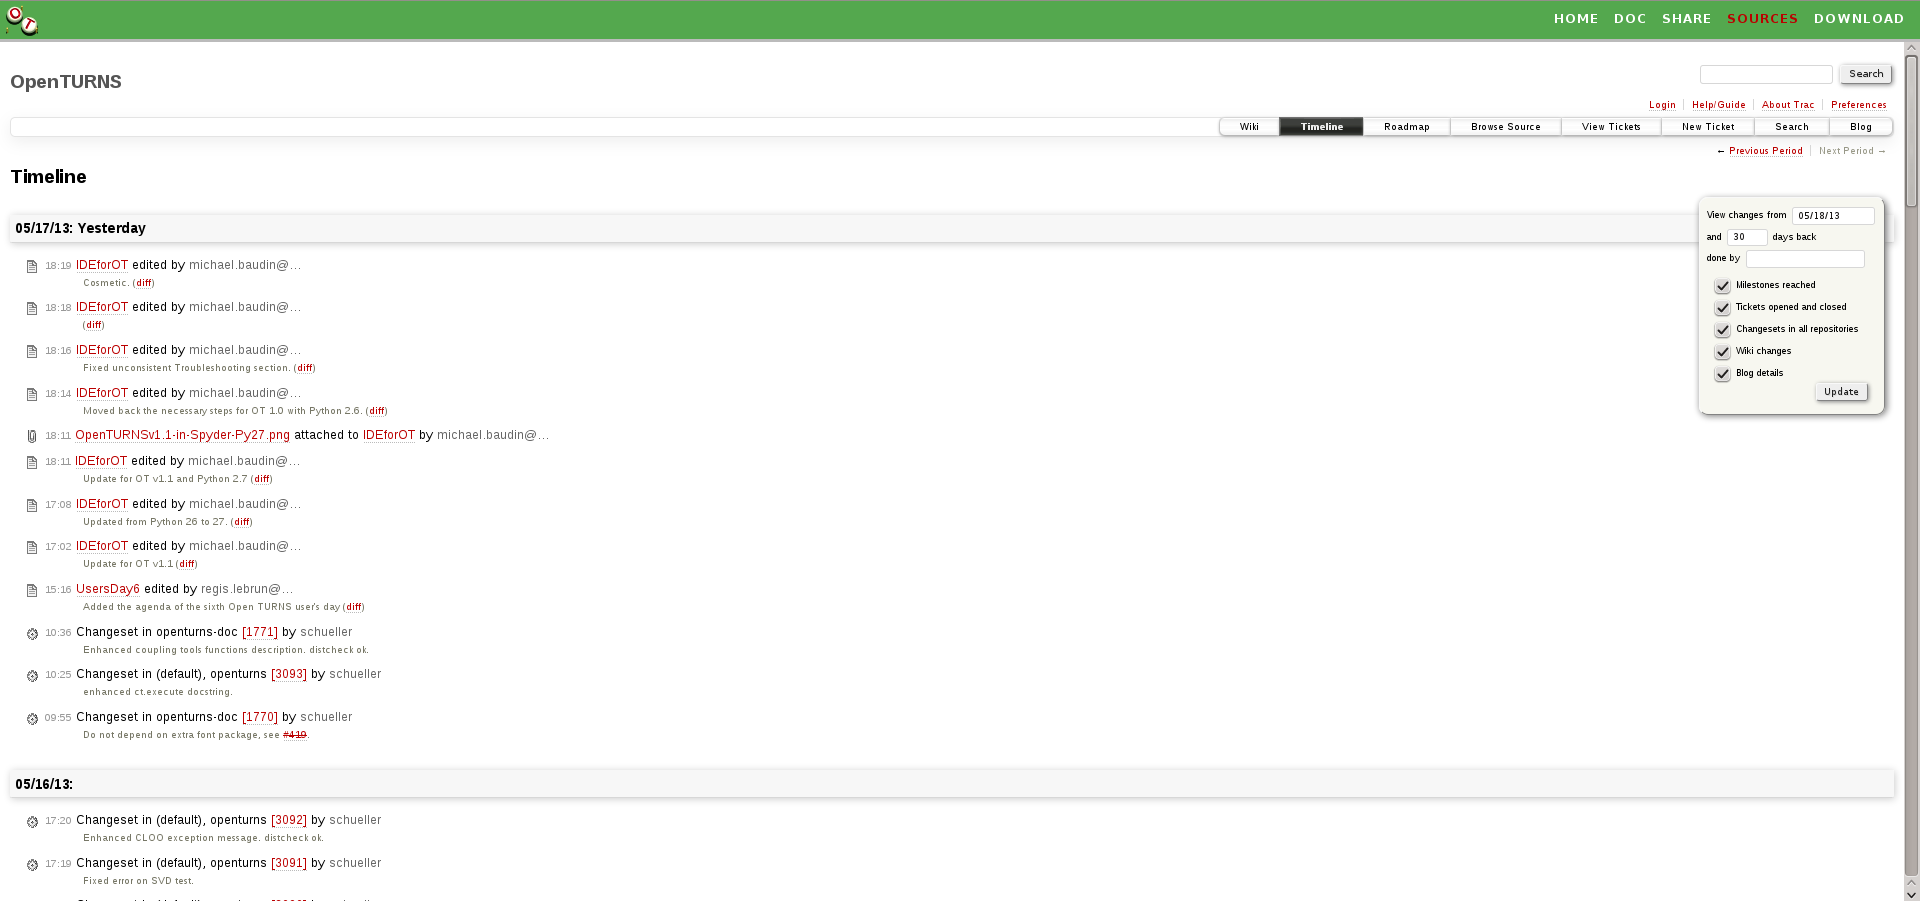
\includegraphics[scale=0.33]{Figures/Timeline.png}
\caption{Trac interface: the timeline}\label{fig:timeline}
\end{center}
\end{figure}

Trac also allows you to explore the vcs repository from your browser at \url{http://trac.openturns.org/browser}; the snapshot \ref{fig:browser} here focuses on one changeset, showing the changes in in files.

\begin{figure}[ht]
\begin{center}
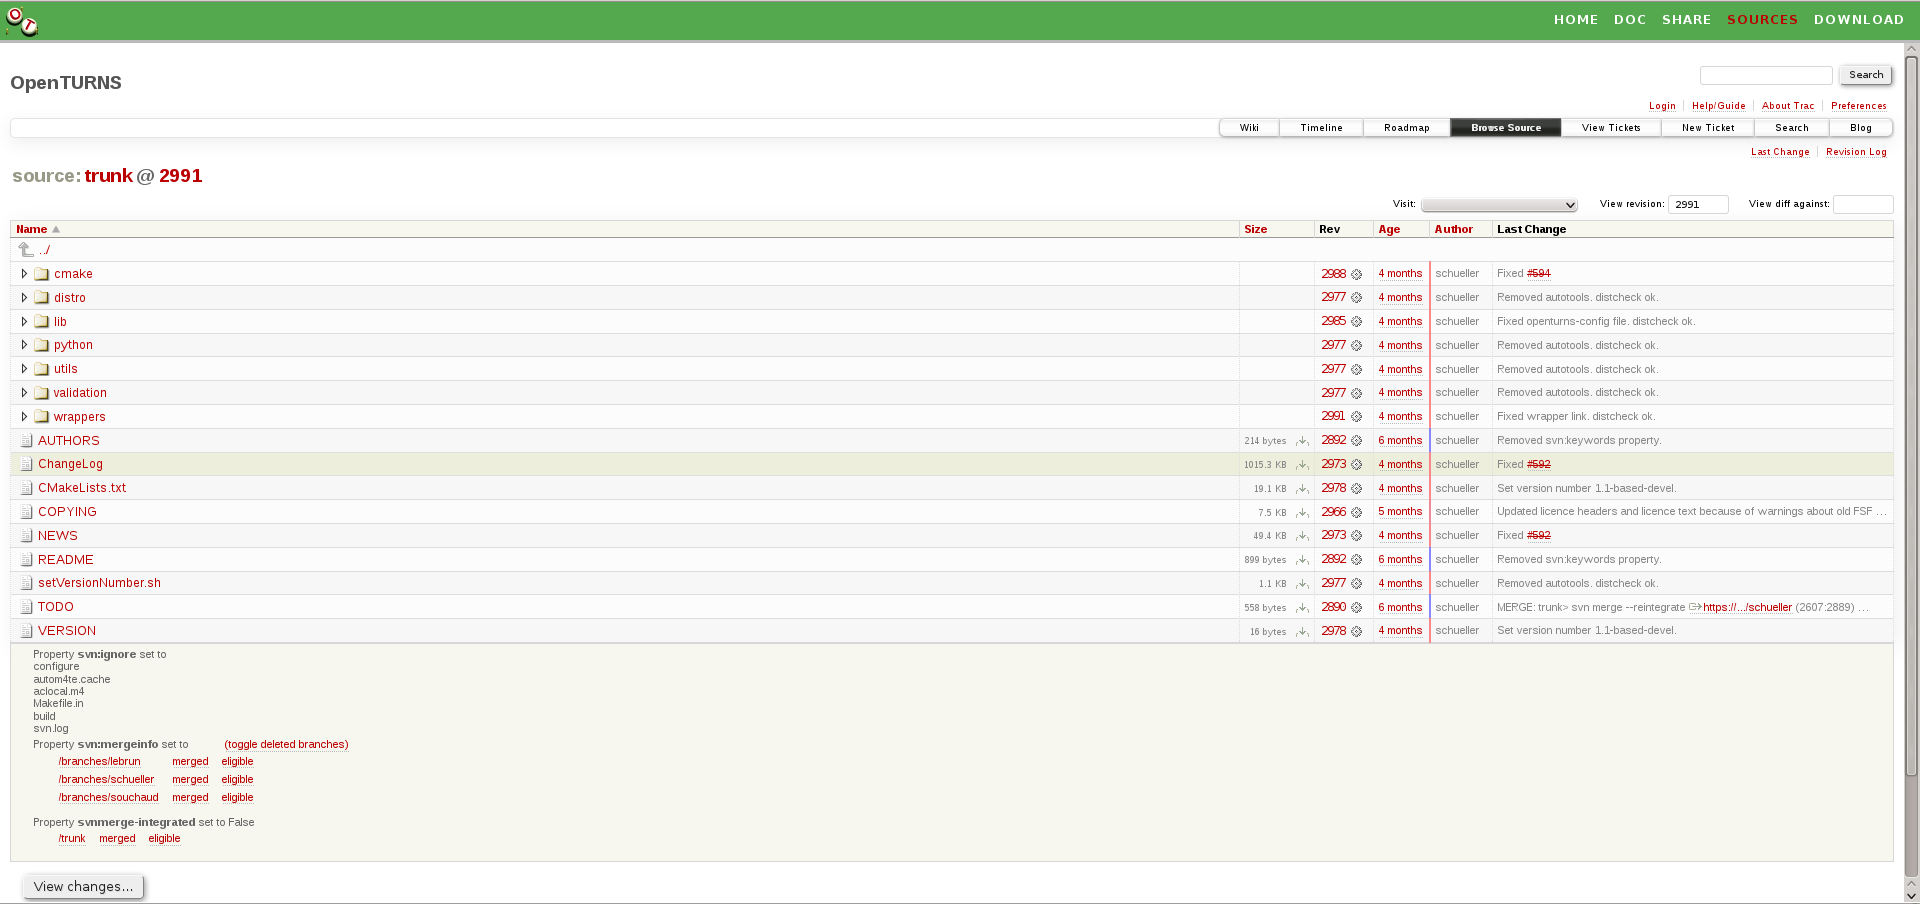
\includegraphics[scale=0.33]{Figures/BrowseSource.png}
\caption{Trac interface: the source browser}\label{fig:browser}
\end{center}

\end{figure}

Trac provides a bug-tracker at \url{http://trac.openturns.org/report}. The snapshot \ref{fig:ticket1} shows the list of active tickets.

\begin{figure}[ht]
\begin{center}
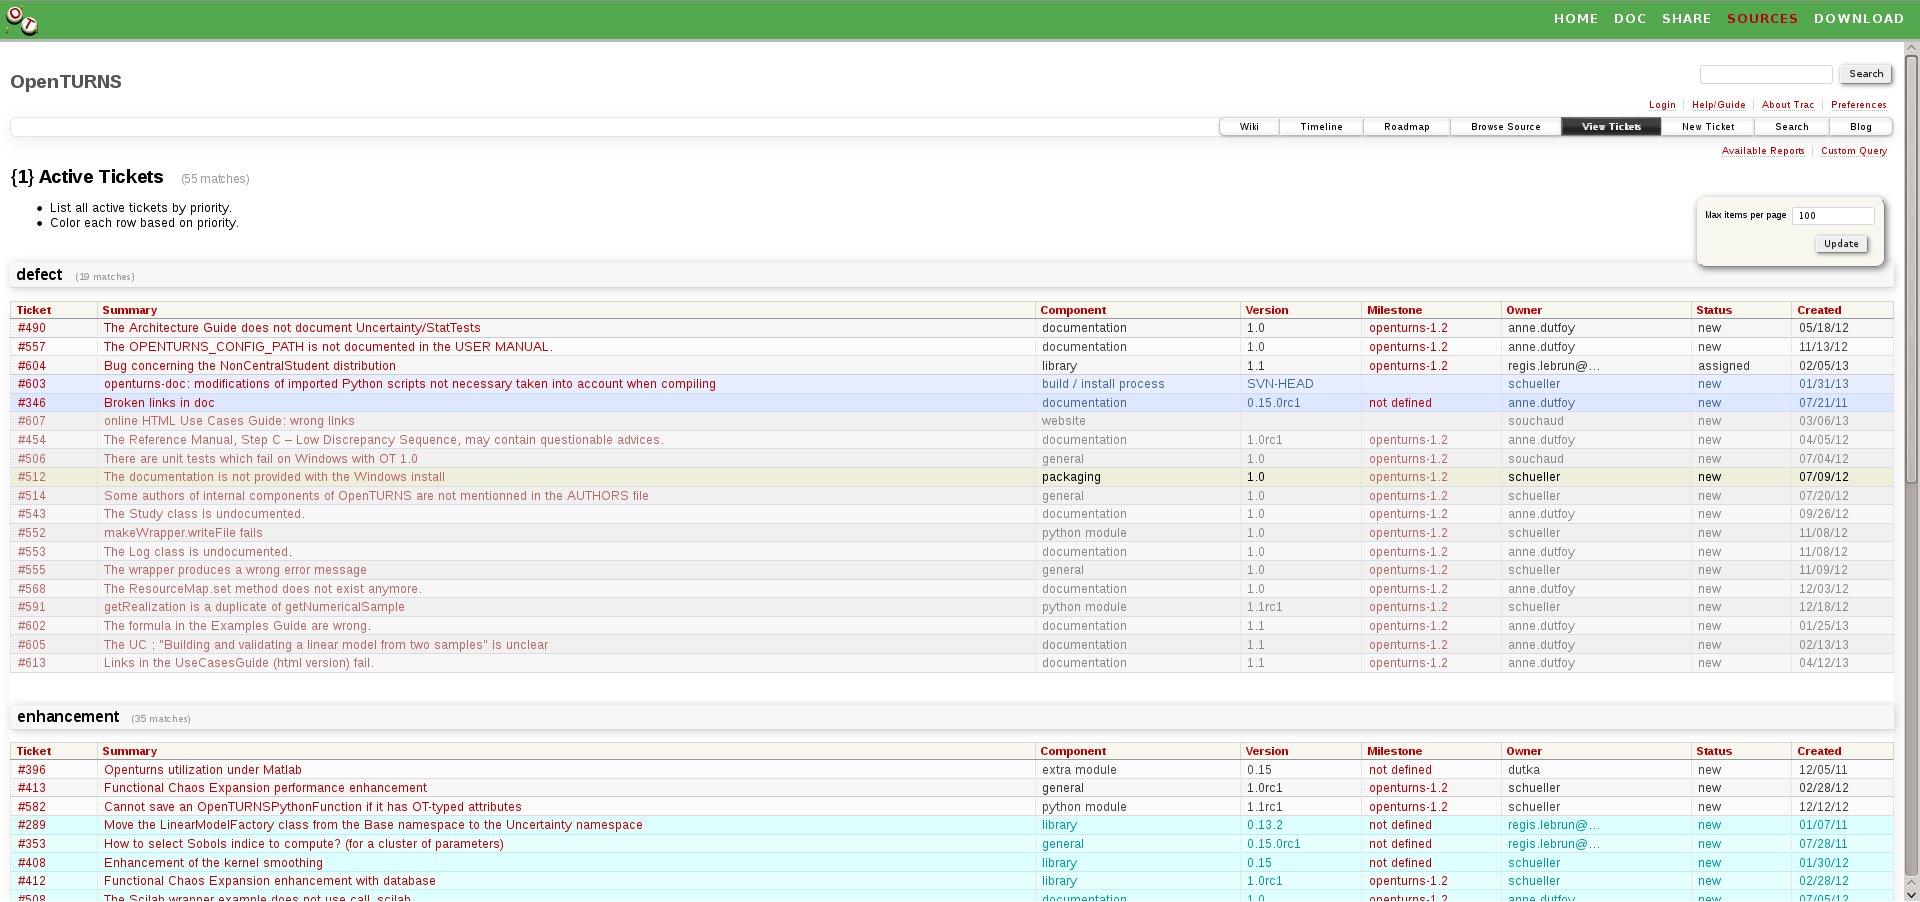
\includegraphics[scale=0.33]{Figures/Tickets1.png}
\caption{Trac interface: the ticket report view}\label{fig:ticket1}
\end{center}

\end{figure}

Each ticket features attributes to help classification, interactive comments and file attachment. Snapshot \ref{fig:ticket2} exposes the details of a ticket.

\begin{figure}[ht]
\begin{center}
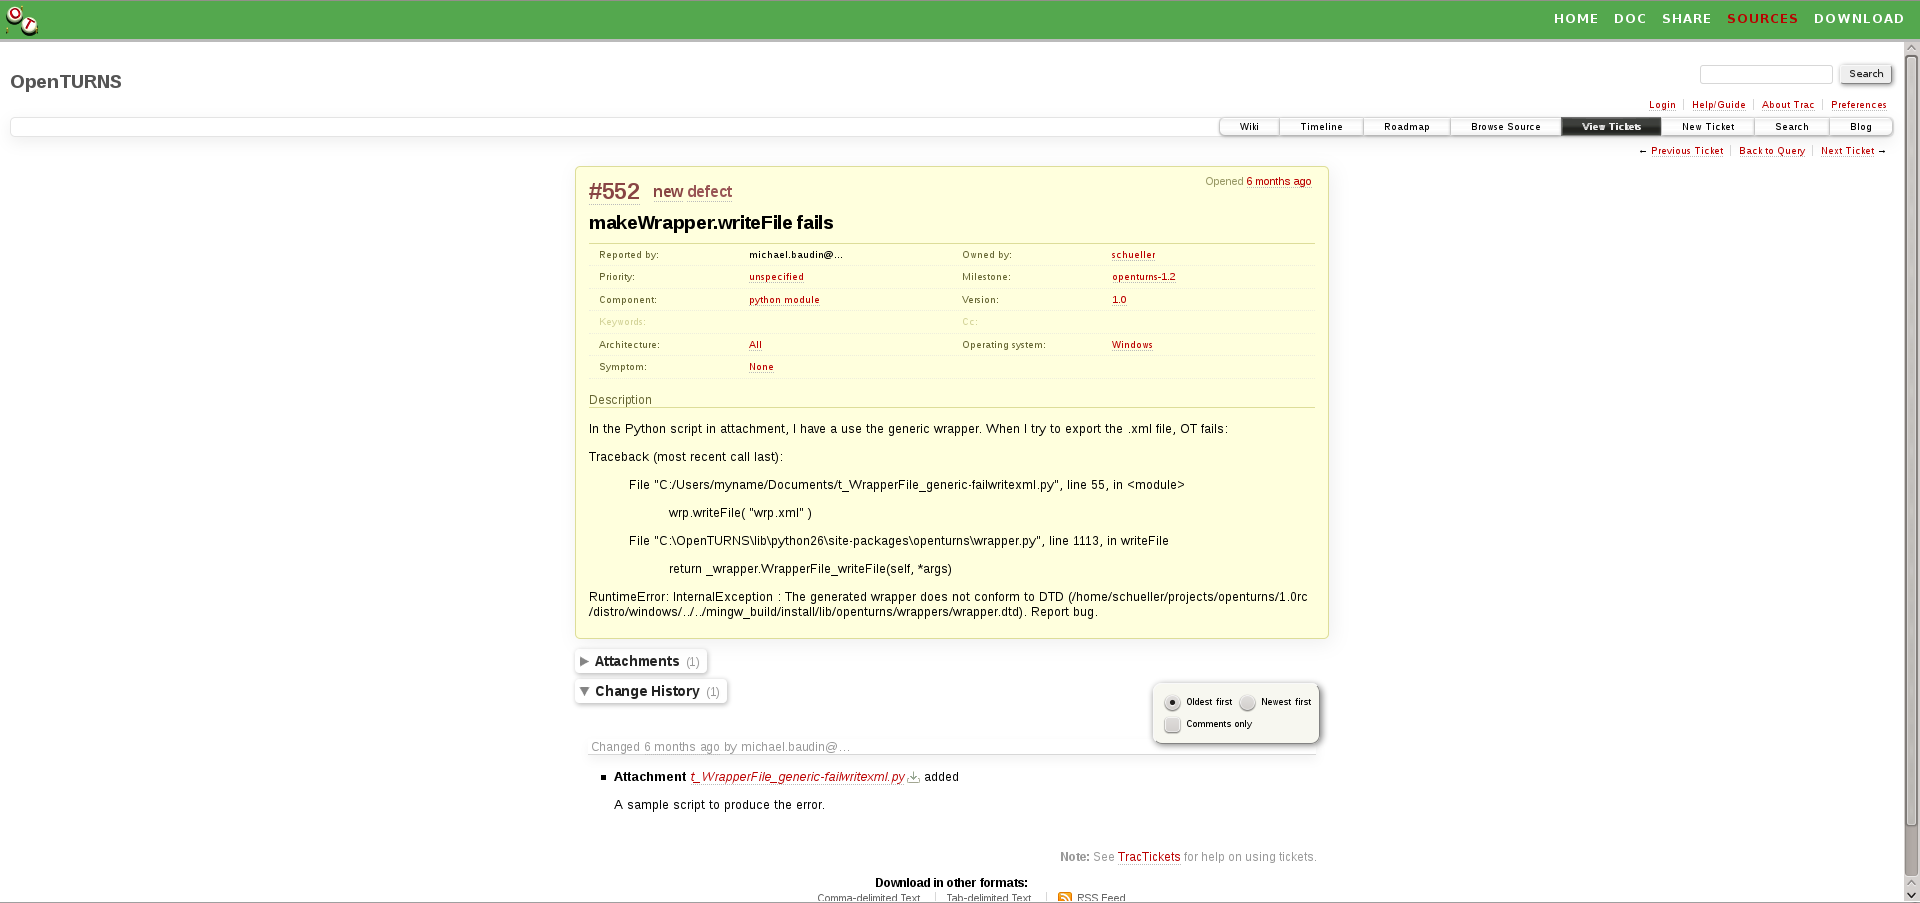
\includegraphics[scale=0.33]{Figures/Tickets2.png}
\caption{Trac interface: details of a ticket report}\label{fig:ticket2}
\end{center}
\end{figure}

\subsection{Other requirements}

\label{namespace}\subsubsection{Namespace}

All the classes of the \OT\ library are accessible within a single namespace named OT and aliased as OpenTURNS. It allows to insulate these classes from classes from another project that could share the same name. Macros are provided to enclose your code in the \OT\ namespace as follow:

\begin{lstlisting}
BEGIN_NAMESPACE_OPENTURNS
// code
END_NAMESPACE_OPENTURNS
\end{lstlisting}

\subsubsection{Internationalization}

The OpenTURNS platform is meant to be widely distributed within the scientific community revolving around probability and statistics, which is essentially an international community. Therefore, the platform should be designed so as to be adjustable to the users, particularly those who do not speak English\footnote{English has been chosen as the native language for the OpenTURNS platform.}.

This involves not using any messages directly in the source code of the platform, but rather to create a resource catalogue that can be loaded, according to the locale setting of the user, when the application is launched.

Another consequence of internationalization is the need for the Unicode extended character set to be used for all strings.

\subsubsection{Accessibility}

The OpenTURNS platform shall be accessible to disabled users. This has implications on the ergonomics and the design of the User Interface, particularly the GUI which should offer keyboard shortcuts for any available function as well as keyboard-based (rather than mouse-based) mechanisms to handle and select objects.


\subsubsection{Programming conventions}

Please refer to appendix \ref{coding_rules}.
